\documentclass[10pt]{article}
\usepackage[a4paper,margin=18mm]{geometry}
\usepackage[T1]{fontenc}\usepackage{lmodern}
\usepackage{amsmath,amssymb,booktabs,array,enumitem}
\usepackage{tikz}\usetikzlibrary{shapes.gates.logic.US,positioning,arrows.meta}
\usepackage[hidelinks]{hyperref}
\setlength{\parindent}{0pt}\setlength{\parskip}{4pt}\setlength{\emergencystretch}{2em}
\newcommand{\mos}[4]{\begin{scope}[shift={(#1,#2)}]
\draw(0,.24)--(0,-.24);\draw(0,.2)--(.25,.2)--(.25,.5);\draw(0,-.2)--(.25,-.2)--(.25,-.5);
\draw(-.16,.23)--(-.16,-.23);
\ifnum#4=1\draw(-.26,0)circle(.06);\draw(-.75,0)--(-.32,0);\else\draw(-.75,0)--(-.16,0);\fi
\node[anchor=east,font=\scriptsize]at(-.76,0){$#3$};\end{scope}}
\newcommand{\gnd}[2]{\draw(#1,#2)--(#1,{#2-.12});\draw({#1-.17},{#2-.12})--({#1+.17},{#2-.12});\draw({#1-.11},{#2-.2})--({#1+.11},{#2-.2});}
\newcommand{\rail}[3]{\draw(#1,#2)--(#1,{#2+.14});\node[above,font=\scriptsize]at(#1,{#2+.14}){$#3$};}
\begin{document}
\begin{center}\large\textbf{2022 Midterm -- Independent Corrected Solutions}\\\normalsize Complete original questions 1--6, 100 points\end{center}
\textbf{Method.} Derivations follow the printed topology and values. The graded handwriting and supplement are comparison sources; accepted marks do not validate a mistaken physical claim. All diagrams are editable TikZ, and the checks use graph/truth or stipulated RC models without process simulation.
\section*{Question 1: concepts (35 points)}
\textbf{(a) Mask transfer.} Prepare the wafer, coat photoresist and soft bake; align the mask and expose; develop the resist; etch the exposed underlying material; strip the remaining resist. Exposure changes the resist and etching transfers its developed pattern into the substrate/layer. The handwritten outline is expanded to include development. \href{https://www.sfu.ca/~gchapman/e495/e495l3l.pdf}{[SFU fabrication lecture]}

\textbf{(b) SOI.} An active silicon layer sits on buried oxide (BOX), above a silicon handle wafer. The insulating BOX isolates it from bulk silicon, reducing source/drain-to-bulk junction area and leakage. Fully depleted SOI additionally improves channel electrostatic control and can reduce off-state leakage. Source/body and drain/body PN junctions can remain in the film; the student's claim of no PN junctions is too strong. Gate and channel leakage are not automatically eliminated. \href{https://www.st.com/content/st_com/en/about/innovation-and-technology/fd-soi.html}{[ST FD-SOI]}

\textbf{(c) Oxidation terminology.} Two actual thermal oxidation methods are dry oxidation and wet oxidation:
\[\mathrm{Si+O_2\to SiO_2},\qquad\mathrm{Si+2H_2O\to SiO_2+2H_2}.\]
The supplied answers alternatively classify oxide formation as thermal oxidation and CVD oxide deposition. Thermal oxidation consumes substrate silicon; CVD deposits an oxide film. CVD is not direct oxidation of the silicon substrate. The original wording does not uniquely choose between thermal variants and oxide-formation processes, so both classifications are stated explicitly. \href{https://www.utep.edu/engineering/nanomil/processes/oxidation_basics.html}{[UTEP oxidation]}, \href{https://www.cleanroom.byu.edu/FilmDeposition}{[BYU growth/deposition]}

\textbf{(d) Static CMOS features.} A valid steady-state input gives full rail-to-rail output restoration and ideally zero DC supply current, because one complementary network is OFF. Practical static power is leakage; both networks can conduct during switching. A single complementary complex gate is inverting, while multistage static CMOS circuits can be noninverting.

\textbf{(e) Static power.} Reverse-biased source/drain-to-body/well PN junctions produce junction leakage; OFF MOS transistors produce subthreshold channel leakage. $P_{static}=V_{DD}I_{leak}$. Replace the handwritten latch-up/BJT answer with subthreshold leakage; latch-up is an abnormal failure condition rather than the intended normal leakage component. \href{https://people.eecs.berkeley.edu/~alanmi/research/timing/papers/lec25_bw_2xp.pdf}{[Berkeley CMOS power]}

\textbf{(f) Pull-up/down polarity.} PMOS drives a strong logic 1 to $V_{DD}$ and NMOS a strong logic 0 to GND. With gate voltages restricted to the supply rails, an NMOS pull-up loses about $V_{tn}$ and a PMOS pull-down stops near $|V_{tp}|$. The normal complementary assignment gives full output swing.

\textbf{(g) High-k.} $C_{ox}=\epsilon_0 k/t_{phys}$. A larger dielectric constant allows a physically thicker insulator at the same gate capacitance/equivalent oxide thickness, reducing direct tunneling while maintaining gate control. Distinguish physical from electrical thickness. \href{https://www.intel.com/pressroom/kits/advancedtech/doodle/ref_HiK-MG/high-k.htm}{[Intel high-k]}

\newpage\section*{Question 1 (continued)}
\textbf{(h) TSV processes.} Via-first fabricates TSVs before CMOS FEOL device fabrication; via-last does so after FEOL and BEOL fabrication. Via-middle, a separate category, occurs after FEOL and before BEOL. Thus the student's ``before BEOL'' definition is insufficiently precise for via-first. \href{https://doi.org/10.1116/6.0000026}{[Burkett et al., TSV tutorial]}

\textbf{(i) Body effect.} In a series nMOS stack, the device nearest the output may have the highest internal source voltage while its body stays at GND. Its source/body reverse bias increases its threshold:
\[V_{tn}=V_{tn0}+\gamma\left(\sqrt{2\phi_F+V_{SB}}-\sqrt{2\phi_F}\right).\]
Larger threshold reduces overdrive and drive current. An analogous reverse source/well bias increases the pMOS threshold magnitude. Connection of a lone transistor drain to the output does not by itself cause severe body effect; this explanation concerns displaced source potentials in a stack. Correct the student's trend to $V_{SB}\uparrow\Rightarrow V_{tn}\uparrow$, with the body fixed at GND. \href{https://www.ece.mcmaster.ca/faculty/bakr/ece2ei4/Lecture16_Web.pdf}{[McMaster MOSFET lecture]}

\textbf{(j) Antenna effect.} A floating conductor attached to a thin gate oxide can collect charge during plasma processing and damage the dielectric. Two fixes: (1) add an antenna protection diode/diffusion discharge path; (2) add a jumper near the gate, moving the long conductor to a later-formed higher metal layer so that a smaller area is attached during vulnerable fabrication steps. Arbitrarily splitting layers without the appropriate process-stage isolation is insufficient. \href{https://skywater-pdk.readthedocs.io/en/main/rules/antenna.html}{[SkyWater rules]}, \href{https://users.ece.northwestern.edu/~haizhou/publications/dac06wang.pdf}{[Wang and Zhou jumper insertion]}

\textbf{(k) Bonding classifications.} Orientation styles are face-to-face, face-to-back and back-to-back; face denotes the active-device/interconnect side and back the substrate side. A separate manufacturing-granularity classification is wafer-to-wafer, die-to-wafer and die-to-die. The original does not specify the classification axis. The graded sheet lists orientations and the supplement lists granularities; neither grading nor one list disproves the other. \href{https://www.hajim.rochester.edu/ece/sites/friedman/Boris_Vaisband_PhD.pdf}{[Vaisband 3D integration]}, \href{https://www.imec-int.com/sites/default/files/2024-06/imec_WP_Monolithic_microsystems_LORES.pdf}{[imec assembly granularity]}

\textbf{(l) Output capacitance.} $C_L=C_{gate,load}+C_{diffusion}+C_{wire}$: receiver input gate capacitances, the driving gate's output-connected drain diffusion/junction capacitances, and routing capacitance to the substrate and neighboring wires. Both supplied lists are valid; receiver gate capacitance is meant here.

\textbf{(m) FinFET types.} Shorted-gate (SG): the two side gates are electrically tied. Independent-gate (IG): the side gates can be controlled separately. Correct the student's expansion ``short gate'' to ``shorted-gate''. \href{https://doi.org/10.1145/2832913}{[Chaudhuri and Jha, FinFET logic]}

Primary references support the physical corrections; the exam source determines the exact question text and marks. The notes' Q1 lettering shifts after an added crosstalk answer, so they were matched by wording.
\newpage\section*{Question 2(a): 8-to-1 transmission-gate multiplexer}
Choose the explicit index convention $k=4s_0+2s_1+s_2$, so $y=x_k$. Build seven 2-to-1 cells in a three-level binary tree: four cells controlled by $s_2$, two by $s_1$, and one by $s_0$. Each cell uses two transmission gates. For its input 0, enable on $\overline s$; for input 1, enable on $s$. Every TG consists of a parallel nMOS/pMOS pair. A bubble marks its pMOS gate.
\begin{center}\begin{tikzpicture}[x=1.1cm,y=.78cm,font=\small]
\draw(-.8,5.775)node[left]{$x_0$}--(.27,5.775);
\draw(-.8,4.125)node[left]{$x_1$}--(.27,4.125);
\draw(-.8,2.4750000000000005)node[left]{$x_2$}--(.27,2.4750000000000005);
\draw(-.8,0.8250000000000011)node[left]{$x_3$}--(.27,0.8250000000000011);
\draw(-.8,-0.8249999999999993)node[left]{$x_4$}--(.27,-0.8249999999999993);
\draw(-.8,-2.4749999999999996)node[left]{$x_5$}--(.27,-2.4749999999999996);
\draw(-.8,-4.124999999999998)node[left]{$x_6$}--(.27,-4.124999999999998);
\draw(-.8,-5.774999999999999)node[left]{$x_7$}--(.27,-5.774999999999999);
\draw(0.27,5.625)rectangle(0.73,5.925000000000001);
\draw(0.5,5.925000000000001)--(0.5,6.035);\draw(0.5,6.075)circle(.04);\draw(0.5,6.115)--(0.5,6.205);
\node[above,font=\scriptsize]at(0.5,6.205){$s_2$};
\draw(0.5,5.625)--(0.5,5.375);\node[below,font=\scriptsize]at(0.5,5.375){$\overline{s_2}$};
\draw(0.73,5.775)--(1.4,5.775)--(1.4,4.95);
\draw(0.27,3.975)rectangle(0.73,4.275);
\draw(0.5,4.275)--(0.5,4.385);\draw(0.5,4.425)circle(.04);\draw(0.5,4.465)--(0.5,4.555);
\node[above,font=\scriptsize]at(0.5,4.555){$\overline{s_2}$};
\draw(0.5,3.975)--(0.5,3.725);\node[below,font=\scriptsize]at(0.5,3.725){$s_2$};
\draw(0.73,4.125)--(1.4,4.125)--(1.4,4.95);
\fill(1.4,4.95)circle(1.5pt);
\draw(0.27,2.3250000000000006)rectangle(0.73,2.6250000000000004);
\draw(0.5,2.6250000000000004)--(0.5,2.7350000000000003);\draw(0.5,2.7750000000000004)circle(.04);\draw(0.5,2.8150000000000004)--(0.5,2.9050000000000007);
\node[above,font=\scriptsize]at(0.5,2.9050000000000007){$s_2$};
\draw(0.5,2.3250000000000006)--(0.5,2.0750000000000006);\node[below,font=\scriptsize]at(0.5,2.0750000000000006){$\overline{s_2}$};
\draw(0.73,2.4750000000000005)--(1.4,2.4750000000000005)--(1.4,1.6500000000000008);
\draw(0.27,0.675000000000001)rectangle(0.73,0.9750000000000011);
\draw(0.5,0.9750000000000011)--(0.5,1.085000000000001);\draw(0.5,1.125000000000001)circle(.04);\draw(0.5,1.1650000000000011)--(0.5,1.255000000000001);
\node[above,font=\scriptsize]at(0.5,1.255000000000001){$\overline{s_2}$};
\draw(0.5,0.675000000000001)--(0.5,0.42500000000000104);\node[below,font=\scriptsize]at(0.5,0.42500000000000104){$s_2$};
\draw(0.73,0.8250000000000011)--(1.4,0.8250000000000011)--(1.4,1.6500000000000008);
\fill(1.4,1.6500000000000008)circle(1.5pt);
\draw(0.27,-0.9749999999999993)rectangle(0.73,-0.6749999999999993);
\draw(0.5,-0.6749999999999993)--(0.5,-0.5649999999999993);\draw(0.5,-0.5249999999999992)circle(.04);\draw(0.5,-0.48499999999999927)--(0.5,-0.3949999999999993);
\node[above,font=\scriptsize]at(0.5,-0.3949999999999993){$s_2$};
\draw(0.5,-0.9749999999999993)--(0.5,-1.2249999999999992);\node[below,font=\scriptsize]at(0.5,-1.2249999999999992){$\overline{s_2}$};
\draw(0.73,-0.8249999999999993)--(1.4,-0.8249999999999993)--(1.4,-1.6499999999999995);
\draw(0.27,-2.6249999999999996)rectangle(0.73,-2.3249999999999997);
\draw(0.5,-2.3249999999999997)--(0.5,-2.215);\draw(0.5,-2.175)circle(.04);\draw(0.5,-2.135)--(0.5,-2.0449999999999995);
\node[above,font=\scriptsize]at(0.5,-2.0449999999999995){$\overline{s_2}$};
\draw(0.5,-2.6249999999999996)--(0.5,-2.8749999999999996);\node[below,font=\scriptsize]at(0.5,-2.8749999999999996){$s_2$};
\draw(0.73,-2.4749999999999996)--(1.4,-2.4749999999999996)--(1.4,-1.6499999999999995);
\fill(1.4,-1.6499999999999995)circle(1.5pt);
\draw(0.27,-4.274999999999999)rectangle(0.73,-3.9749999999999983);
\draw(0.5,-3.9749999999999983)--(0.5,-3.8649999999999984);\draw(0.5,-3.8249999999999984)circle(.04);\draw(0.5,-3.7849999999999984)--(0.5,-3.694999999999998);
\node[above,font=\scriptsize]at(0.5,-3.694999999999998){$s_2$};
\draw(0.5,-4.274999999999999)--(0.5,-4.524999999999999);\node[below,font=\scriptsize]at(0.5,-4.524999999999999){$\overline{s_2}$};
\draw(0.73,-4.124999999999998)--(1.4,-4.124999999999998)--(1.4,-4.949999999999998);
\draw(0.27,-5.924999999999999)rectangle(0.73,-5.624999999999998);
\draw(0.5,-5.624999999999998)--(0.5,-5.514999999999999);\draw(0.5,-5.474999999999999)circle(.04);\draw(0.5,-5.434999999999999)--(0.5,-5.344999999999999);
\node[above,font=\scriptsize]at(0.5,-5.344999999999999){$\overline{s_2}$};
\draw(0.5,-5.924999999999999)--(0.5,-6.174999999999999);\node[below,font=\scriptsize]at(0.5,-6.174999999999999){$s_2$};
\draw(0.73,-5.774999999999999)--(1.4,-5.774999999999999)--(1.4,-4.949999999999998);
\fill(1.4,-4.949999999999998)circle(1.5pt);
\draw(2.27,4.8)rectangle(2.73,5.1000000000000005);
\draw(2.5,5.1000000000000005)--(2.5,5.21);\draw(2.5,5.25)circle(.04);\draw(2.5,5.29)--(2.5,5.38);
\node[above,font=\scriptsize]at(2.5,5.38){$s_1$};
\draw(2.5,4.8)--(2.5,4.55);\node[below,font=\scriptsize]at(2.5,4.55){$\overline{s_1}$};
\draw(1.4,4.95)--(2.27,4.95);
\draw(2.73,4.95)--(3.4,4.95)--(3.4,3.3000000000000007);
\draw(2.27,1.5000000000000009)rectangle(2.73,1.8000000000000007);
\draw(2.5,1.8000000000000007)--(2.5,1.9100000000000008);\draw(2.5,1.9500000000000008)circle(.04);\draw(2.5,1.9900000000000009)--(2.5,2.080000000000001);
\node[above,font=\scriptsize]at(2.5,2.080000000000001){$\overline{s_1}$};
\draw(2.5,1.5000000000000009)--(2.5,1.2500000000000009);\node[below,font=\scriptsize]at(2.5,1.2500000000000009){$s_1$};
\draw(1.4,1.6500000000000008)--(2.27,1.6500000000000008);
\draw(2.73,1.6500000000000008)--(3.4,1.6500000000000008)--(3.4,3.3000000000000007);
\fill(3.4,3.3000000000000007)circle(1.5pt);
\draw(2.27,-1.7999999999999994)rectangle(2.73,-1.4999999999999996);
\draw(2.5,-1.4999999999999996)--(2.5,-1.3899999999999995);\draw(2.5,-1.3499999999999994)circle(.04);\draw(2.5,-1.3099999999999994)--(2.5,-1.2199999999999995);
\node[above,font=\scriptsize]at(2.5,-1.2199999999999995){$s_1$};
\draw(2.5,-1.7999999999999994)--(2.5,-2.0499999999999994);\node[below,font=\scriptsize]at(2.5,-2.0499999999999994){$\overline{s_1}$};
\draw(1.4,-1.6499999999999995)--(2.27,-1.6499999999999995);
\draw(2.73,-1.6499999999999995)--(3.4,-1.6499999999999995)--(3.4,-3.299999999999999);
\draw(2.27,-5.099999999999999)rectangle(2.73,-4.799999999999998);
\draw(2.5,-4.799999999999998)--(2.5,-4.689999999999999);\draw(2.5,-4.649999999999999)circle(.04);\draw(2.5,-4.6099999999999985)--(2.5,-4.519999999999999);
\node[above,font=\scriptsize]at(2.5,-4.519999999999999){$\overline{s_1}$};
\draw(2.5,-5.099999999999999)--(2.5,-5.349999999999999);\node[below,font=\scriptsize]at(2.5,-5.349999999999999){$s_1$};
\draw(1.4,-4.949999999999998)--(2.27,-4.949999999999998);
\draw(2.73,-4.949999999999998)--(3.4,-4.949999999999998)--(3.4,-3.299999999999999);
\fill(3.4,-3.299999999999999)circle(1.5pt);
\draw(4.27,3.150000000000001)rectangle(4.73,3.4500000000000006);
\draw(4.5,3.4500000000000006)--(4.5,3.5600000000000005);\draw(4.5,3.6000000000000005)circle(.04);\draw(4.5,3.6400000000000006)--(4.5,3.730000000000001);
\node[above,font=\scriptsize]at(4.5,3.730000000000001){$s_0$};
\draw(4.5,3.150000000000001)--(4.5,2.900000000000001);\node[below,font=\scriptsize]at(4.5,2.900000000000001){$\overline{s_0}$};
\draw(3.4,3.3000000000000007)--(4.27,3.3000000000000007);
\draw(4.73,3.3000000000000007)--(5.4,3.3000000000000007)--(5.4,8.881784197001252e-16);
\draw(4.27,-3.449999999999999)rectangle(4.73,-3.149999999999999);
\draw(4.5,-3.149999999999999)--(4.5,-3.039999999999999);\draw(4.5,-2.999999999999999)circle(.04);\draw(4.5,-2.959999999999999)--(4.5,-2.8699999999999988);
\node[above,font=\scriptsize]at(4.5,-2.8699999999999988){$\overline{s_0}$};
\draw(4.5,-3.449999999999999)--(4.5,-3.699999999999999);\node[below,font=\scriptsize]at(4.5,-3.699999999999999){$s_0$};
\draw(3.4,-3.299999999999999)--(4.27,-3.299999999999999);
\draw(4.73,-3.299999999999999)--(5.4,-3.299999999999999)--(5.4,8.881784197001252e-16);
\fill(5.4,8.881784197001252e-16)circle(1.5pt);
\draw(5.4,8.881784197001252e-16)--(6.0,8.881784197001252e-16)node[right]{$y$};
\end{tikzpicture}\end{center}\begin{center}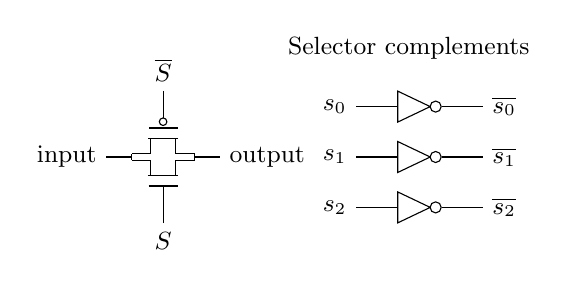
\begin{tikzpicture}[x=.8cm,y=.8cm,font=\small]
\begin{scope}[shift={(0,.3)},rotate=-90]\mos{0}{0}{}{1}\end{scope}
\begin{scope}[shift={(0,-.3)},rotate=90]\mos{0}{0}{}{0}\end{scope}
\draw(-.5,-.05)--(-.5,.05);\draw(.5,-.05)--(.5,.05);\draw(-.9,0)--(-.5,0);\draw(.5,0)--(.9,0);
\node[left]at(-.9,0){input};\node[right]at(.9,0){output};
\node[above]at(0,1.05){$\overline S$};\node[below]at(0,-1.05){$S$};
\begin{scope}[shift={(3.9,0)}]
\node[above]at(0,1.4){Selector complements};
\foreach\i/\h in {0/.8,1/0,2/-.8}{\node[not gate US,draw](s\i)at(0,\h){};\draw(s\i.input)--++(-.65,0)node[left]{$s_{\i}$};\draw(s\i.output)--++(.65,0)node[right]{$\overline{s_{\i}}$};}
\end{scope}
\end{tikzpicture}\\TG detail and the three selector-complement generators.\end{center}
Each selected data path contains three ON TGs; exactly one of $x_0,\ldots,x_7$ connects to $y$ for a settled selection code. There are 14 TGs (28 pass transistors), plus the three CMOS inverters shown (6 transistors) to generate selector complements: 34 total. Tie pass nMOS bodies to GND and pMOS bodies to $V_{DD}$. The graded decoder-style arrangement can also select one input, but does not justify a linearly growing unbuffered delay.

\newpage\section*{Question 2(b): unbuffered delay scaling}
With $N$ selection bits there are $2^N$ data inputs and $N$ successive TG levels along a selected tree path. Treat the ON TGs as $R_{TG}$ and each visited-node parasitic as $C_{int}$; let external load be $C_L$. The Elmore delay scale is
\[\tau\simeq R_{TG}C_{int}\frac{N(N+1)}2+N R_{TG}C_L.\]
Upstream resistances must charge all downstream node capacitances, so internal RC delay grows quadratically with unbuffered depth: $\tau=O(N^2)$ when each node capacitance is comparable. For three levels, $\tau\simeq6R_{TG}C_{int}+3R_{TG}C_L$. A chain of restoring buffers is a different case, for which comparable stage delays can sum linearly. The graded sheet's $T\propto N$ claim omits the distributed capacitive loading; the supplement recognizes the square dependence. No absolute delay is determined because TG resistance and node/load capacitance values are not supplied.

\section*{Question 2(c): complete the three multiplexers}
Read the printed 0/1 port labels; handwritten letters around Figure 1(b) are not constraints. Shannon expansion on $B$ gives
\[F=\overline B(C+D)+B(A+D).\]
Use $D$ to select between $C$ and 1 for the upper mux, and between $A$ and 1 for the lower mux. Select the upper/lower outputs with $B$:
\begin{center}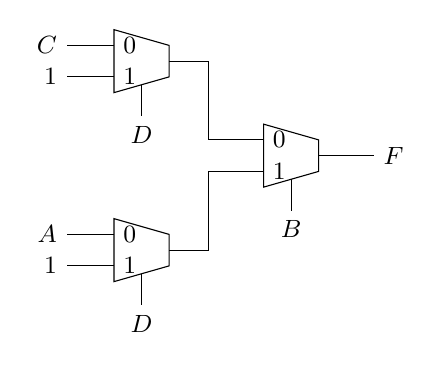
\begin{tikzpicture}[font=\small]
\draw(-.4,.8)--(-.4,1.6)--(.3,1.4)--(.3,1.0)--cycle;
\node at(-.2,1.4){0};\node at(-.2,1){1};
\draw(-.4,-1.6)--(-.4,-.8)--(.3,-1.0)--(.3,-1.4)--cycle;
\node at(-.2,-1){0};\node at(-.2,-1.4){1};
\draw(1.5,-.4)--(1.5,.4)--(2.2,.2)--(2.2,-.2)--cycle;
\node at(1.7,.2){0};\node at(1.7,-.2){1};
\draw(.3,1.2)--(.8,1.2)|-(1.5,.2);\draw(.3,-1.2)--(.8,-1.2)|-(1.5,-.2);
\draw(2.2,0)--(2.9,0)node[right]{$F$};
\draw(-0.4,1.4)--(-1.0,1.4)node[left]{$C$};\draw(-0.4,1)--(-1.0,1)node[left]{$1$};\draw(-0.4,-1)--(-1.0,-1)node[left]{$A$};\draw(-0.4,-1.4)--(-1.0,-1.4)node[left]{$1$};\draw(-0.05,0.9)--(-0.05,0.5)node[below]{$D$};\draw(-0.05,-1.5)--(-0.05,-1.9)node[below]{$D$};\draw(1.85,-0.3)--(1.85,-0.7)node[below]{$B$};\end{tikzpicture}\end{center}
For $B=0$, the upper result is $C+D$; for $B=1$, the lower result is $A+D$. Hence $F=AB+\overline{B}C+D$. This agrees with the graded completion after mapping the port order. The verifier checks all 16 input combinations.

\newpage\section*{Question 3(a): minimum-delay buffer with original equal-width devices}
The load ratio is $H=C_L/C_g=2.98\,\mathrm{pF}/1\,\mathrm{fF}=2980$. Let $N$ inverter stages have equal n/p width factors $s_i$ relative to $W_{min}$, with $s_0=1$ so NAND A sees exactly $C_g$. The dashed buffer is noninverting, so $N$ must be even. For fixed $N$, equal interstage ratios give $s_i=f^i$, where $f=H^{1/N}$; the last load is $H C_g$.
\begin{center}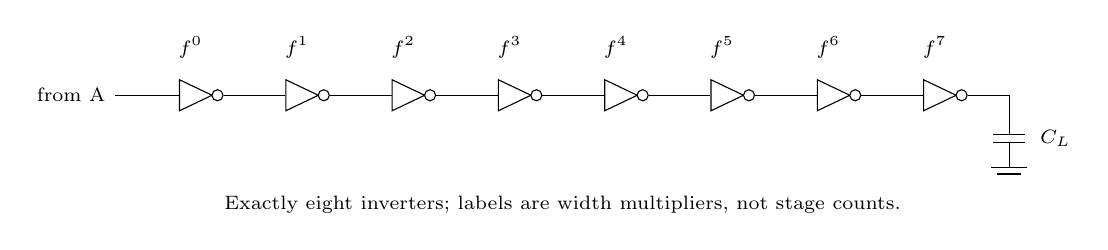
\begin{tikzpicture}[x=1.35cm,y=1cm,font=\scriptsize]
\foreach\i in {0,...,7}{\node[not gate US,draw](i\i)at(\i,0){};\node[above]at(\i,.35){$f^{\i}$};}
\draw(i0.input)--++(-.6,0)node[left]{from A};
\foreach\i in {0,...,6}{\pgfmathtruncatemacro{\j}{\i+1}\draw(i\i.output)--(i\j.input);}
\draw(i7.output)--(7.7,0);\draw(7.7,0)--(7.7,-.5);\draw(7.55,-.5)--(7.85,-.5);\draw(7.55,-.6)--(7.85,-.6);\draw(7.7,-.6)--(7.7,-.8);\gnd{7.7}{-.8};\node[right]at(7.9,-.55){$C_L$};
\node[below]at(3.5,-1.15){Exactly eight inverters; labels are width multipliers, not stage counts.};
\end{tikzpicture}\end{center}
Each nMOS resistance is $R/s_i$ and each equal-width pMOS is $2R/s_i$ because $\mu_n=2\mu_p$. Over an even chain, either transition direction visits $N/2$ nMOS and $N/2$ pMOS pull paths. Thus
\[T_{unmodified}=\frac32N H^{1/N}RC_g.\]
For arbitrary positive stage efforts $f_i$ with $\prod_i f_i=H$, the two direction delays sum to $3RC_g\sum_i f_i$. Consequently their maximum is at least $\frac32RC_g\sum_i f_i\ge\frac32NH^{1/N}RC_g$ by AM--GM. Equal efforts attain this bound for an even chain, establishing the geometric taper for the worst-case objective despite unequal n/p mobility.
The continuous minimum occurs near $N=\ln H\simeq8$; comparing admissible even counts gives $\boxed{N=8}$ and $f=2980^{1/8}\simeq2.71817\simeq e$. Both n/p widths in stage $i=0,\ldots,7$ are $f^iW_{min}/L_{min}$. Exactly eight inverters are required: stage 0 through stage 7. The supplement's extra stage 8 makes nine inverters and reverses the required polarity. The graded sheet's eight-stage geometric taper is retained with explicit indexing and resistance accounting.

\newpage\section*{Question 3(b): fixed nMOS, balanced pMOS and changed loads}
To make each inverter's rise/fall times equal, double its pMOS width while keeping its nMOS unchanged:
\[W_{n,i}=f^iW_{min},\qquad W_{p,i}=2f^iW_{min}.\]
With $C_g$ defined as the total input capacitance of a minimum inverter whose two devices both have $W_{min}$, a single minimum transistor contributes $C_g/2$. The modified input gate capacitance is consequently
\[C_{in,i}=\frac{C_g}{2}(f^i+2f^i)=\frac32f^iC_g.\]
Both pull resistances are now $R/f^i$. The first seven stages drive modified next-stage gate loads; the eighth still drives the unchanged external $C_L$. Therefore
\[\boxed{T_{modified}=\left[\frac32(N-1)+1\right]fRC_g=\frac{3N-1}{2}fRC_g.}\]
For $N=8$, $T_{modified}=11.5fRC_g\simeq31.25899RC_g$. Using the paper's rounded $e=2.7$ gives about $31.05RC_g$. The last stage must not receive the 1.5 gate-load multiplier because $C_L$ is fixed, external capacitance.

\textbf{Input-load consequence.} The first inverter now presents $1.5C_g$ to NAND A. Keeping its nMOS fixed, balancing the pMOS and keeping the original $C_g$ input load cannot all hold simultaneously. Part(b) specifies the fixed nMOS modification; the changed upstream load is stated rather than silently claiming part(a)'s first-load condition remains satisfied. Upstream NAND delay is outside the source's marked buffer delay $T$.

The handwritten $T=NRC$ omits geometric stage effort and the altered gate loads. The verifier records all eight actual widths, gate capacitances and load terms; it also compares even stage counts for part(a). No new process-dependent timing parameters are assumed.

\newpage\section*{Question 4: Schmitt-type n-side feedback}
Before output fall, $V_{out}=1.2\,\mathrm V$ turns feedback N2 on. The source topology and waveform are:
\begin{center}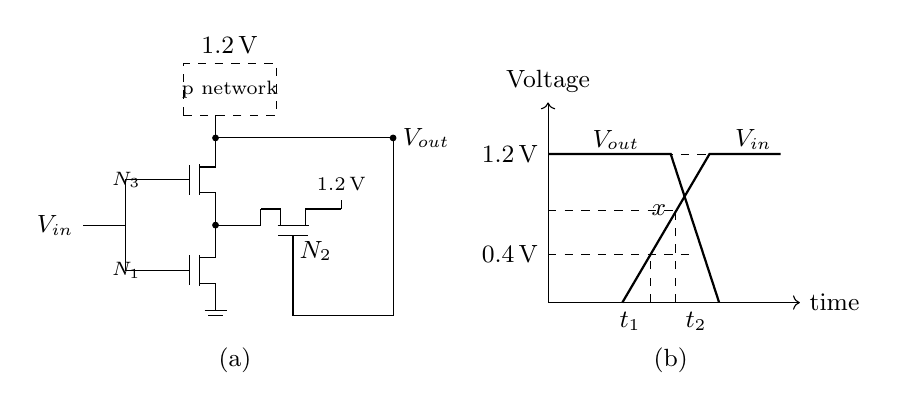
\begin{tikzpicture}[scale=.82,font=\small]
\draw[dashed](-.25,3.5)rectangle(1.2,4.3);\node[font=\scriptsize]at(.47,3.9){p network};\node[above]at(.47,4.3){$1.2\,\mathrm V$};
\draw(.25,3.5)--(.25,3.0);\mos{0}{2.5}{N_3}{0}\mos{0}{1.1}{N_1}{0}
\draw(.25,2)--(.25,1.6);\gnd{.25}{.6}
\draw(-.75,2.5)--(-1.15,2.5)--(-1.15,1.1)--(-.75,1.1);\draw(-1.15,1.8)--(-1.8,1.8)node[left]{$V_{in}$};
\draw(.25,3.15)--(3,3.15)node[right]{$V_{out}$};\fill(.25,3.15)circle(1.5pt);
\begin{scope}[shift={(1.45,1.8)},rotate=90]\mos{0}{0}{}{0}\end{scope}
\draw(.25,1.8)--(.95,1.8)--(.95,2.05);\fill(.25,1.8)circle(1.5pt);
\draw(1.95,2.05)--(2.2,2.05);\rail{2.2}{2.05}{1.2\,\mathrm V};\node at(1.8,1.4){$N_2$};
\draw(1.45,1.05)--(1.45,.4)--(3,.4)--(3,3.15);\fill(3,3.15)circle(1.5pt);
\begin{scope}[xshift=1.4cm]
\draw[->](4.0,.6)--(7.9,.6)node[right]{time};\draw[->](4,.6)--(4,3.7)node[above]{Voltage};
\draw[dashed](4,2.9)--(6.9,2.9);\node[left]at(4,2.9){$1.2\,\mathrm V$};
\draw[dashed](4,1.35)--(6.2,1.35);\node[left]at(4,1.35){$0.4\,\mathrm V$};
\draw[thick](4,2.9)--(5.9,2.9)--(6.65,.6);\node at(5.05,3.12){$V_{out}$};
\draw[thick](5.15,.6)--(6.5,2.9)--(7.6,2.9);\node at(7.18,3.13){$V_{in}$};
\draw[dashed](5.58,.6)--(5.58,1.35);\draw[dashed](5.98,.6)--(5.98,2.03);\node[below left]at(5.58,.6){$t_1$};\node[below right]at(5.98,.6){$t_2$};
\draw[dashed](4,2.03)--(5.98,2.03);\node[left]at(5.98,2.03){$x$};
\node at(5.9,-.3){(b)};\end{scope}\node at(.55,-.3){(a)};
\end{tikzpicture}\\Figure 3: (a) A CMOS logic gate. (b) Waveforms of $V_{in}$ and $V_{out}$.\end{center}
With the stated ON resistances, N1 and N2 set their common internal node to
\[V_a=1.2\frac{R}{R+2R}=0.4\,\mathrm V.\]
The upper series device N3 begins conducting when $V_{in}-V_a=V_{tn}=0.4\,\mathrm V$, giving
\[\boxed{x=V_{in}(t_2)=0.8\,\mathrm V.}\]
At $t_1$, $V_{in}=0.4\,\mathrm V$ and N1 reaches threshold. For the open interval $t_1<t<t_2$:
\begin{center}\begin{tabular}{lccc}\toprule
Device&$V_{GS}$&$V_{DS}$&Region\\\midrule
N1&$V_{in}$&$0.4\,\mathrm V$&Saturation: $V_{DS}\ge V_{GS}-V_{tn}$\\
N2&$0.8\,\mathrm V$&$0.8\,\mathrm V$&Saturation\\
N3&$V_{in}-0.4\,\mathrm V$&$0.8\,\mathrm V$&Cutoff: $V_{GS}<V_{tn}$\\\bottomrule
\end{tabular}\end{center}
At $t_2$, N3 is at threshold and N1 at the saturation/triode boundary; conduction then triggers output fall. These are the source's constant-ON-resistance estimates, not an exact MOS transient calculation. The supplied .8V and saturation/saturation/cutoff conclusions agree after fixing inconsistent intermediate voltage labels. N2 has $V_{GS}=V_{DS}=.8V$, not an overdrive of.8V; its overdrive is.4V.

\newpage\section*{Question 5: the rail-fed/pass XOR}
The left TG is enabled by $\overline A$: pMOS gate $A$, nMOS gate $\overline A$. The right pair has common gate $B$, pMOS source $A$, and nMOS source $\overline A$. Thus
\[A=0:\ y=B,\qquad A=1:\ y=\overline B,\qquad\boxed{y=A\oplus B}.\]
\begin{center}\begin{tabular}{cccl}\toprule
$A$&$B$&$y$&Valid settled drive path\\\midrule
0&0&0&TG connects $B=0$; right pMOS also connects $A=0$\\
0&1&1&TG passes $B=1$ strongly; right nMOS connects $\overline A=1$\\
1&0&1&TG off; right pMOS connects $A=1$\\
1&1&0&TG off; right nMOS connects $\overline A=0$\\\bottomrule
\end{tabular}\end{center}
The complete TG avoids a threshold-loss problem for the two $A=0$ cases; the active right device passes a strong 1 or 0 for $A=1$. Under ideal settled input rails, all four outputs are correct.
\begin{center}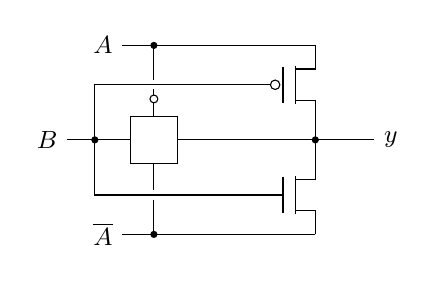
\begin{tikzpicture}[font=\small]\begin{scope}[shift={(0,0)}]
\draw(-.2,3)--(2.25,3);\node[left]at(-.2,3){$A$};\draw(-.2,.6)--(2.25,.6);\node[left]at(-.2,.6){$\overline A$};
\mos{2}{2.5}{}{1}\mos{2}{1.1}{}{0}\draw(2.25,2)--(2.25,1.6);\draw(2.25,1.8)--(3,1.8)node[right]{$y$};\fill(2.25,1.8)circle(1.3pt);
\draw(-.1,1.5)rectangle(.5,2.1);\draw(.2,2.1)--(.2,2.27);\draw(.2,2.32)circle(.05);\draw(.2,2.37)--(.2,2.44);\draw(.2,2.56)--(.2,3);\fill(.2,3)circle(1.3pt);
\draw(.2,1.5)--(.2,1.16);\draw(.2,1.04)--(.2,.6);\fill(.2,.6)circle(1.3pt);
\draw(.5,1.8)--(2.25,1.8);\draw(-.9,1.8)--(-.1,1.8)node[pos=0,left]{$B$};\fill(-.55,1.8)circle(1.3pt);
\draw(-.55,1.8)--(-.55,2.5)--(1.25,2.5);\draw(-.55,1.8)--(-.55,1.1)--(1.25,1.1);

\end{scope}\end{tikzpicture}\end{center}

\textbf{Weakness.} There is no separate restoring stage supplied directly by fixed $V_{DD}$/GND. Output drive comes through the pass network or through A/$\overline A$ input drivers acting as rails. Output resistance, fan-out capability and noise propagation depend on those input drivers; switched sources/body bias and finite input/complement arrival times can worsen delay or create transient glitches. The TG also provides no input isolation. The student's statement ``no driving ability'' is too strong: finite conductive paths exist, but it lacks independent full restoring drive. A restoring buffer pair could preserve XOR polarity while increasing load-driving capability; no extra devices are needed to identify the requested function and weaknesses.

\newpage\section*{Question 6(a): positive function $F=X(Y+Z)+XW$}
Factor $F=X(Y+Z+W)$. Build $U=\overline{X(Y+Z+W)}$ with nMOS $X$ in series with parallel $Y,Z,W$, and the dual pMOS network; add a static output inverter to obtain $F=\overline U$.
\begin{center}\begin{tikzpicture}[x=.75cm,y=.75cm,font=\small]
\mos{0}{2.55}{X}{1}
\draw(.25,3.05)--(.25,4.3)--(3.25,4.3);\rail{1.6}{4.3}{V_{DD}};\draw(.25,2.05)--(.25,.25);
\mos{3}{3.45}{Y}{1}
\mos{3}{2.35}{Z}{1}
\mos{3}{1.25}{W}{1}
\draw(3.25,4.3)--(3.25,3.95);
\draw(3.25,2.95)--(3.25,2.85);
\draw(3.25,1.85)--(3.25,1.75);
\draw(3.25,0.75)--(3.25,.25);
\mos{0}{-.75}{X}{0}
\draw(.25,.25)--(.25,-.25);\draw(.25,-1.25)--(.25,-1.55);
\draw(.25,-1.55)--(4.25,-1.55);\draw(.25,-3.05)--(4.25,-3.05);
\mos{0}{-2.3}{Y}{0}\draw(0.25,-1.55)--(0.25,-1.8);\draw(0.25,-2.8)--(0.25,-3.05);
\mos{2}{-2.3}{Z}{0}\draw(2.25,-1.55)--(2.25,-1.8);\draw(2.25,-2.8)--(2.25,-3.05);
\mos{4}{-2.3}{W}{0}\draw(4.25,-1.55)--(4.25,-1.8);\draw(4.25,-2.8)--(4.25,-3.05);
\gnd{1.3}{-3.05};
\draw(.25,.25)--(4.85,.25);\fill(3.25,.25)circle(1.5pt);\node[above]at(4.35,.25){$U$};
\mos{7}{2}{U}{1}\mos{7}{-1}{U}{0}
\rail{7.25}{2.5}{V_{DD}};\gnd{7.25}{-1.5};\draw(7.25,1.5)--(7.25,-.5);
\draw(4.85,.25)--(5.7,.25)--(5.7,2)--(6.25,2);\draw(5.7,.25)--(5.7,-1)--(6.25,-1);\fill(5.7,.25)circle(1.5pt);
\draw(7.25,.25)--(8.2,.25)node[right]{$F$};\fill(7.25,.25)circle(1.5pt);
\end{tikzpicture}\end{center}
This requires 8 core devices plus 2 inverter devices, using only the original primary inputs. Tie all pMOS bodies to $V_{DD}$ and all nMOS bodies to GND. The complemented-input student construction can be valid if explicit input inverters are included, as the supplement attempts; the factored original-input implementation avoids assuming free complements. The checker verifies all 16 assignments and PUN/PDN rail exclusivity.

\newpage\section*{Question 6(b): equivalent inverter for the specified transition}
Here $F=\overline{X(Y+Z)}$, with every original transistor $W/L$. Fixing $X=1,Y=0$ leaves $F=\overline Z$ for the source sequence $101\to100\to101$, so $F:0\to1\to0$.
\begin{center}\begin{tabular}{lcc}\toprule
Output transition&Conducting original path&Equivalent resistance\\\midrule
Rise ($101\to100$)&pMOS Y and Z in series&$2R_p$\\
Fall ($100\to101$)&nMOS X and Z in series&$2R_n$\\\bottomrule
\end{tabular}\end{center}
Equivalent resistance doubles when width halves. An inverter driven by $Z$, with both its pMOS and nMOS width $W/2$ and unchanged length $L$, therefore represents these two active paths:
\begin{center}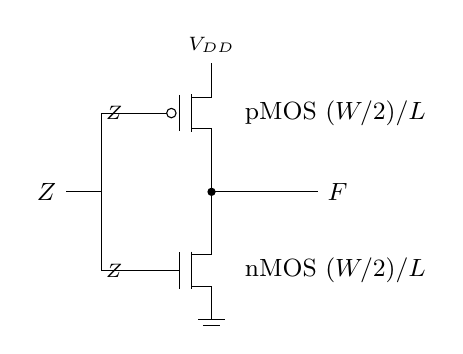
\begin{tikzpicture}[font=\small]
\mos{0}{2}{Z}{1}\mos{0}{0}{Z}{0}\rail{.25}{2.5}{V_{DD}};\gnd{.25}{-.5};\draw(.25,1.5)--(.25,.5);\draw(.25,1)--(1.6,1)node[right]{$F$};\fill(.25,1)circle(1.5pt);
\draw(-.75,2)--(-1.15,2)--(-1.15,0)--(-.75,0);\draw(-1.15,1)--(-1.6,1)node[left]{$Z$};
\node[right]at(.55,2){pMOS $(W/2)/L$};\node[right]at(.55,0){nMOS $(W/2)/L$};
\end{tikzpicture}\end{center}
For symbolic output load $C_o$, $\boxed{t_r\simeq2R_pC_o,\quad t_f\simeq2R_nC_o}$. $R_p,R_n$ refer to their original $W/L$ devices. Q6 does not independently specify a mobility ratio or output capacitance, so these remain symbolic. If the $\mu_n=2\mu_p$ convention is additionally applied, $R_p=2R_n$ and $t_r=2t_f$; this conditional ratio is not needed for the width-equivalence answer. This is an ON-resistance equivalent for the stated transition, not a claim of matching all internal capacitances or body biases. The handwritten half-width equivalent inverter agrees with the transition-specific derivation.

\section*{Reproducibility}
Run \texttt{python verify.py}. Saved CSV/JSON checks cover eight mux selection codes, 16 Shannon inputs, RC ladder scaling, even buffer stage counts and each modified load, Schmitt-region sample points, four XOR routes, 16 CMOS truth states and the equivalent-inverter transition sequence. No simulated waveforms or device-model measurements are claimed.
\end{document}
